\section{សំណួរ លំហាត់អនុវត្តន៍ និងកិច្ចការផ្ទះ}
\begin{enumerate}
	\item ចូររកកំប៉ូសង់នៃវុិចទ័រក្នុងករណីនីមួយៗខាងក្រោម៖
	\begin{enumerate}[k,2]
		\item 
		\begin{tikzpicture}
			\begin{scope}
				\coordinate[label=above:$\overrightarrow{A}$] (A) at (1.5,2);
				\coordinate (O) at (0,0);
				\draw[->] (-.5,0) -- (4,0);
				\draw[->, blue] (O) -- (A);
				\draw[->] (0,-.3) -- (0,4);
				\coordinate[label=below:$x$] (X) at (4,0);
				\coordinate[label=left:$y$] (Y) at (0,4);
				\pic [draw, ->, "$65^\circ$", angle eccentricity=1.5, angle radius=1cm] {angle= X--O--A};
				\node at (1.8,1.5) {$38 m$};
			\end{scope}
		\end{tikzpicture}
		\item 
			\begin{tikzpicture}
				\begin{scope}
					\coordinate[label=above:$\overrightarrow{B}$] (B) at (-1.5,2.8);
					\coordinate (O) at (0,0);
					\draw[->] (-3,0) -- (2,0);
					\draw[->, blue] (O) -- (B);
					\draw[->] (0,-.3) -- (0,4);
					\coordinate[label=below:$x$] (X) at (2,0);
					\coordinate[label=left:$y$] (Y) at (0,4);
					\pic [draw, ->, "$135^\circ$", angle eccentricity=1.5, angle radius=1cm] {angle= X--O--B};
					\node at (-1.5,1.5) {$33 m$};
				\end{scope}
			\end{tikzpicture}
		\item 
			\begin{tikzpicture}
				\begin{scope}
					\coordinate[label=below:$\overrightarrow{C}$] (C) at (-2,-2);
					\coordinate (O) at (0,0);
					\draw[->] (-3,0) -- (2,0);
					\draw[->, blue] (O) -- (C);
					\draw[->] (0,-2.5) -- (0,2);
					\coordinate[label=below:$x$] (X) at (2,0);
					\coordinate[label=left:$y$] (Y) at (0,2);
					\pic [draw, ->, "$214^\circ$", angle eccentricity=1.5, angle radius=.8cm] {angle= X--O--C};
					\node at (-.8,-2) {$43 m$};
				\end{scope}
			\end{tikzpicture}
		\item 
			\begin{tikzpicture}
				\begin{scope}
					\coordinate[label=below:$\overrightarrow{D}$] (D) at (2,-1);
					\coordinate (O) at (0,0);
					\draw[->] (-3,0) -- (3,0);
					\draw[->, blue] (O) -- (D);
					\draw[->] (0,-2) -- (0,2);
					\coordinate[label=below:$x$] (X) at (3,0);
					\coordinate[label=left:$y$] (Y) at (0,2);
					\pic [draw, ->, "$338^\circ$", angle eccentricity=1.5, angle radius=.8cm] {angle= X--O--D};
					\node at (1,-1) {$35 m$};
				\end{scope}
			\end{tikzpicture}
	\end{enumerate}
	\item ចូររកកុំប៉ូសង់តាមអ័ក្សអាប់ស៊ីស និងអរដោនេនៃវ៉ិចទ័រខាងក្រោម៖
	\begin{enumerate}[k,2]
		\item 
		\begin{tikzpicture}
			\begin{scope}
			\coordinate[label=above:$\overrightarrow{v}$] (V) at (1.5,2);
			\coordinate (O) at (0,0);
			\draw[->] (-.5,0) -- (4,0);
			\draw[->, blue] (O) -- (V);
			\draw[->] (0,-.3) -- (0,4);
			\coordinate[label=below:$x$] (X) at (4,0);
			\coordinate[label=left:$y$] (Y) at (0,4);
			\pic [draw, ->, "$45^\circ$", angle eccentricity=1.5, angle radius=1cm] {angle= X--O--V};
			\node at (1.8,1.5) {$2 m$};
			\end{scope}
		\end{tikzpicture}
		\item 
		\begin{tikzpicture}
			\begin{scope}
			\coordinate[label=above:$\overrightarrow{u}$] (U) at (-1.5,2.8);
			\coordinate (O) at (0,0);
			\draw[->] (-3,0) -- (2,0);
			\draw[->, blue] (O) -- (U);
			\draw[->] (0,-.3) -- (0,4);
			\coordinate[label=below:$x$] (X) at (2,0);
			\coordinate[label=left:$y$] (Y) at (0,4);
			\pic [draw, ->, "$120^\circ$", angle eccentricity=1.5, angle radius=1cm] {angle= X--O--U};
			\node at (-1.5,1.5) {$4m$};
			\end{scope}
		\end{tikzpicture} 
	\end{enumerate}
	\item គេឲ្យបម្លាស់ទីពីរគឺ $\overrightarrow{r}_{1}=\left(6.00\vec{i}+3.00\vec{j}\right)m$ និង $\overrightarrow{r}_{2}=\left(4.00\vec{i}+5.00\vec{j}\right)m$។\\ ចូរគណនា $\overrightarrow{r}_{1}+\overrightarrow{r}_{2},~\overrightarrow{r}_{1}-\overrightarrow{r}_{2},~2\overrightarrow{r}_{1}-\overrightarrow{r}_{2}$ និងម៉ូឌុលរបស់វាផង។
	\item អ្នកចង់រកកំពស់ដើមឈើតែមិនអាចវាស់ដោយផ្ទាល់បានទេ។ អ្នកឈរចម្ងាយ $50.0m$ ពីដើមឈើហើយកំណត់ថា បន្ទាត់នៃការមើលឃើញពីដីទៅដល់កំពូលនៃដើមឈើបង្កើតបានមុំ $25.0^\circ$ ជាមួយនឹងដី។ តើដើមឈើមានកំពស់ប៉ុន្មាន?
	\begin{figure}[H]
		\centering
		\begin{tikzpicture}
			\begin{scope}
				\coordinate (O) at (0,0);
				\coordinate (A) at (-10,-2);
				\coordinate (B) at (0,-2);
				\coordinate (C) at (0,2);
				\node at (O) {
\includegraphics[scale=.5]{tree}};
				\node at (-10.2,-1.1) {
\includegraphics[scale=.3]{girl}};
				\draw[line width=1.5pt] (A) -- (B);
				\draw[line width=1.5pt] (B) -- (C);
				\draw[line width=1.5pt] (C) -- (A);
				\pic [draw, "$25.0^\circ$", angle eccentricity=1.5, angle radius=2cm] {angle= B--A--C};
				\draw[->, line width=1.5pt] (.5,-.5) -- (.5,2);
				\draw[->, line width=1.5pt] (.5,-1) -- (.5,-2);
				\node at (.5, -.8) {$h$};
				\draw[->, line width=1.5pt] (-5.8,-2.5) -- (-10,-2.5);
				\draw[->, line width=1.5pt] (-4.2,-2.5) -- (0,-2.5);
				\node at (-5, -2.5) {$50.0m$};
			\end{scope}
		\end{tikzpicture}
		\caption{លំហាត់ទី៤}
	\end{figure}
	\item រកបម្លាស់ទីតាមអ័ក្សអាប់ស៊ីស និងអ័ក្សអរដោនេនៃបម្លាស់ទី $100.0m$ របស់កំពូលវីរបុរសម្នាក់បានហោះចេញពីកំពូលនៃដំបូលអាគារមួយដូចបានបង្ហាញក្នុងរូប។
	\begin{figure}[H]
		\centering
		\begin{tikzpicture}[scale=1.2]
			\coordinate (O) at (-.9,1.4);
			\coordinate[label=right:$x$] (X) at (2,1.4);
			\coordinate[label=left:$y$] (Y) at (-.9,2.5);
			\coordinate (M) at (1.2,-.2);
			\coordinate (B) at (-2,0);
			\node[rotate=-36] at (-.3,.5) {$100.0m$};
			\node at (1,0) {
\includegraphics[scale=.25]{super-hero}};
			\node at (B) {
\includegraphics[scale=.7]{building}};
			\draw[->] (O) -- (Y);
			\draw[->] (O) -- (X);
			\draw[->, draw=cyan, line width=2pt] (O) -- (M);
			\pic [draw, "$30.0^\circ$", angle eccentricity=1.5, angle radius=1cm] {angle= M--O--X};
		\end{tikzpicture}
		\caption{លំហាត់ទី៥}
	\end{figure}
%	\item យន្ដហោះមួយបានហោះចេញពីជំរុំមូលដ្ឋានទៅបឹង $A$ ចម្ងាយ $289km$ ក្នុងទិសដៅ $20.0^\circ$ ពីជើងឆៀងកើត។ បន្ទាប់ពីទម្លាក់ឧបករណ៍សង្គ្រោះវាបន្តហោះទៅបឹង $B$ ដែលមានចម្ងាយ $190km$ នៅ $30.0^\circ$ ខាងលិចភាគខាងជើងពីបឹង $A$។\\ គូសរូបបញ្ជាក់ដើម្បីកំណត់ចំងាយ និងទិសដៅពីបឹង $B$ ទៅជំរុំមូលដ្ឋាន។
	\item អ្នកជម្ងឺម្នាក់គាត់បានកាត់ឆ្អឹងដៃ ហើយដៃរបស់គាត់បានចងទាញដូចបង្ហាញក្នុងរូប។ ខ្សែទាំងពីរនោះត្រូវបានទាញដោយវ៉ិចទ័រកម្លាំងពីរគឺ $\overrightarrow{A}$ និង $\overrightarrow{B}$ ដែលមានតម្លៃស្មើៗគ្នា និងបង្កើតកម្លាំងផ្គួបដែលមានលើដៃអ្នកជម្ងឺនោះគឺ $5.60N$។ គណនាកម្លាំងដែលអនុវត្តលើខ្សែនីមួយៗ។
	\begin{figure}[H]
		\centering
		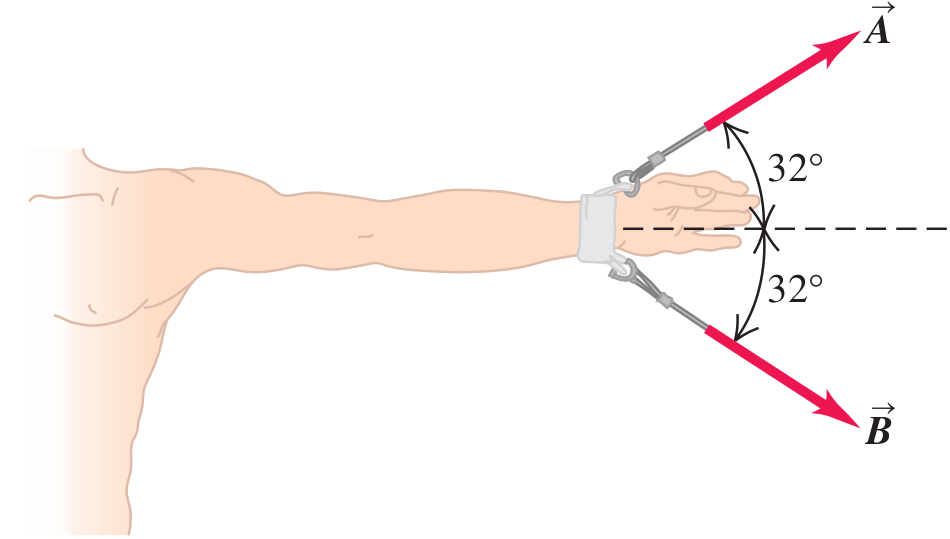
\includegraphics[scale=.2]{patient}
		\caption{លំហាត់ទី៧}
	\end{figure}
	\item ឡានមួយត្រូវបានទាញដោយកម្លាំងពីរតាមរយៈខ្សែពួរពីរខ្សែ(ដូចរូប) ខ្សែទាំងពីរនេះផ្គុំគ្នាបានមុំ $30.0^\circ $។ តម្លៃនៃកម្លាំងដែលអនុវត្តលើខ្សែនីមួយៗគឺ $2900N$។ គណនាកម្លាំងផ្គួបដែលមានអំពើលើរថយន្តនេះ។
	\begin{figure}[H]
		\centering
		\begin{tikzpicture}
			\coordinate (O) at (1.7,0);
			\coordinate[label=above:$2900N$] (F1) at (4,1);
			\coordinate[label=below:$2900N$] (F2) at (4,-1);
			\node at (0,0) {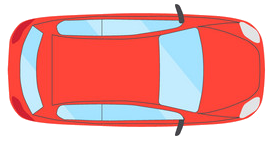
\includegraphics[scale=.4]{car1}};
			\draw[->, line width = 2pt] (O) -- (F1);
			\draw[dashed, line width = 1pt] (O) -- (4.2,0);
			\draw[->, line width = 2pt] (O) -- (F2);
			\pic [draw, "$30.0^\circ$", angle eccentricity=1.5, angle radius=2cm] {angle= F2--O--F1};
		\end{tikzpicture}
		\caption{លំហាត់ទី៨}
	\end{figure}
	\item វ៉ិចទ័រនៃកម្លាំងពីរ $\overrightarrow{F}_{1}$ និង $\overrightarrow{F}_{2}$ មានអំពើលើវត្ថុមួយដែល $F_{1}=20.0N$ និង $F_{2}=15.0N$។\\ ចូរគណនាកម្លាំងផ្គួបដែលមានលើវត្ថុនេះក្នុងករណី \emph{\kml ក,ខ} និង \emph{\kml គ}។
	\begin{enumerate}[k,3]
		\item \begin{tikzpicture}
		\begin{scope}
			\coordinate (O) at (0,0);
			\coordinate[label=right:$\overrightarrow{F}_{1}$] (F1) at (2,0);
			\coordinate[label=above:$\overrightarrow{F}_{2}$] (F2) at (0,2);
			\draw [->, line width =2pt] (O) -- (F1);
			\draw [->, line width =2pt] (O) -- (F2); 
			\shade [ball color=cyan!20!white] (O) circle [radius=10pt];
			\node at (O) {$m$};
			\pic [draw, "$90.0^\circ$", angle eccentricity=1.7, angle radius=.7cm] {angle= F1--O--F2};
		\end{scope}
		\end{tikzpicture}
		\item \begin{tikzpicture}
			\begin{scope}
				\coordinate (O) at (0,0);
				\coordinate[label=right:$\overrightarrow{F}_{1}$] (F1) at (2,0);
				\coordinate[label=above:$\overrightarrow{F}_{2}$] (F2) at (2,2);
				\draw [->, line width =2pt] (O) -- (F1);
				\draw [->, line width =2pt] (O) -- (F2); 
				\shade [ball color=cyan!20!white] (O) circle [radius=10pt];
				\node at (O) {$m$};
				\pic [draw, "$60.0^\circ$", angle eccentricity=1.5, angle radius=1cm] {angle= F1--O--F2};
			\end{scope}
		\end{tikzpicture}
		\item \begin{tikzpicture}
			\begin{scope}
				\coordinate (O) at (0,0);
				\coordinate[label=right:$\overrightarrow{F}_{1}$] (F1) at (2,0);
				\coordinate[label=above:$\overrightarrow{F}_{2}$] (F2) at (-2,2);
				\draw [->, line width =2pt] (O) -- (F1);
				\draw [->, line width =2pt] (O) -- (F2); 
				\shade [ball color=cyan!20!white] (O) circle [radius=10pt];
				\node at (O) {$m$};
				\pic [draw, "$120.0^\circ$", angle eccentricity=1.5, angle radius=.8cm] {angle= F1--O--F2};
			\end{scope}
		\end{tikzpicture}
	\end{enumerate}
\end{enumerate}